\section{Evaluation}
\label{sec:Evaluation}

\subsection{Datasets}

We evaluate our method on two public benchmarks that together cover synthetic, large-scale variation and high-fidelity real scans.  First, Anomaly-ShapeNet is a synthetic point-cloud benchmark built on top of ShapeNetCoreV2 and intended to provide diverse, controllable defect examples for 3D anomaly detection \cite{li2024towards,chang2015shapenet}.  The released benchmark used in this paper contains 1,600 samples across 40 object categories. The authors synthesize six realistic defect types, namely bulge, concavity, hole, break, bending, and crack, with the anomalous region occupying about one to ten percent of the points in affected samples.  Defects are created using Blender sculpting tools and the corresponding point-level ground truth masks are generated by geometric comparison tools and exported with CloudCompare \cite{li2024towards}.

Second, Real3D-AD is a high-precision, real-scan dataset collected for industrial 3D anomaly detection and benchmarking \cite{liu2023real3d}. Real3D-AD contains 1,254 scanned objects spanning 12 categories (for example, airplane, car, candybar, diamond, seahorse and toffees).  The point clouds are high density, with per-object point counts ranging from tens of thousands to on the order of two million points.  Scans were captured using a blue-light structured-light scanner (PMAX-S130) on a rotating turntable to obtain full 360 degree coverage; defects were labeled using a CloudCompare-based pipeline that leverages octree comparison plus manual verification to produce per-point anomaly masks \cite{liu2023real3d}.  The dataset is organized in a prototype-based training setup: each class provides a small set of pristine prototypes for training and separate test folders containing both normal and defective scans together with ground-truth masks and text annotations, which makes Real3D-AD suitable for evaluating prototype-driven and registration-based anomaly methods.

\subsection{Implementation Details}
\label{sec:impl}

All experiments\footnote{Code and dataset: \url{https://github.com/hoangcuongbk80/Mamba3dAD}} were conducted on a workstation equipped with four NVIDIA RTX 3090 GPUs. All input scans were preprocessed with voxel-grid filtering to ensure tractable memory and computation. The voxel size was \(0.0005\,\mathrm{m}\) for Real3D-AD and \(0.001\,\mathrm{m}\) for Anomaly-ShapeNet. Each point cloud was translated to zero mean and scaled to unit radius after voxelization. The augmentation pipeline ran on the fly prior to patch extraction. The augmentations comprised random yaw rotation uniformly sampled from \([0,2\pi)\), isotropic Gaussian jitter with standard deviation \(\sigma_{\mathrm{jitter}}=0.005\,\mathrm{m}\) clipped at \(2\sigma_{\mathrm{jitter}}\), uniform scaling in \([0.95,1.05]\), random point dropout up to \(5\%\), and random translation with magnitude at most \(0.002\,\mathrm{m}\). The implementation applied augmentations consistently within each forward pass so that patch identity remained stable across backbone layers during that pass.

Patch extraction used Farthest Point Sampling (FPS) to select \(M=256\) patch centers by default. Each center gathered up to \(K_{\max}=512\) nearest neighbors, and the effective neighborhood size was \(K_{\mathrm{eff}}=\min(K_{\max},N)\), where \(N\) denotes the number of points remaining after voxelization. The implementation used \(K_{\mathrm{eff}}=256\) as an alternative default for memory-constrained runs. Each neighborhood was encoded by a lightweight PointNet-style encoder followed by a two-layer positional-encoding MLP to produce embeddings in \(\mathbb{R}^D\). The Transformer backbone was Point-MAE pretrained on ShapeNet and remained frozen in all experiments. The implementation collected tokens from all \(L=6\) encoder layers with embedding dimension \(D=768\). The implementation mapped the \(T\) tokens to a reduced ordered slot bank of size \(S\) for scalability. The default slot count was \(S=1024\). The implementation computed intra-layer descriptors \(E\in\mathbb{R}^{T\times d_a}\) with \(d_a=128\) and learned a set of \(S\) slot queries \(Q\in\mathbb{R}^{S\times d_a}\). Token-slot affinities were obtained via a factorized dot product between \(E\) and \(Q\) with a learned per-slot bias, and the resulting affinities were converted to a numerically stabilized soft-assignment matrix \(P\in[0,1]^{T\times S}\) by the Sinkhorn normalization. Ordered slot features were aggregated using the soft assignments in \(P\). The Sinkhorn normalization employed conservative numerical stabilizations. The implementation subtracted column-wise maxima prior to exponentiation and executed Sinkhorn iterations in log-space for large matrices. The default temperature was \(\tau=0.2\) and the default iteration count was \(K_{\mathrm{sink}}=8\). The implementation performed 64-bit accumulation for normalization when \(T>5000\) or \(S>2048\). The locality bandwidth used unit-radius coordinates with \(\sigma_p=0.05\). The stability constants were \(\epsilon_{\mathrm{ent}}=\epsilon_{\mathrm{norm}}=10^{-6}\). The GSAS regularization weights were \(\alpha_{\mathrm{ent}}=10^{-2}\) and \(\alpha_{\mathrm{loc}}=10^{-1}\), and these values were validated on held-out data. For very long sequences the implementation provided a blockwise-assignment fallback that partitions tokens spatially and executes GSAS per block to reduce peak memory.

Each ordered slot was assigned a spatial coordinate computed as the normalized \(P\)-weighted mean of the contributing patch centers. The implementation supplied this coordinate to the positional-encoding MLP to produce a positional embedding \(e_s\in\mathbb{R}^D\) for each slot. The code maintained a consistent mapping among tokens, patch indices, and slots to enable accurate reprojection and visualization. The Mamba adapter processed the ordered slot sequence of length \(S\). The adapter latent state dimension was \(S_h=256\). The implementation parameterized the transition matrix \(A\) as a scaled orthonormal operator with a learnable scalar initialized to \(0.9\) and with spectral norm constrained to \(0.95\). The input and output projection matrices \(B\), \(C\) and the residual projection \(D\) used Kaiming normal initialization. The implementation applied layer normalization to the recurrent state and a gated residual connection between recurrent and residual pathways to stabilize dynamics. The adapter executed in linear time with respect to \(S\) and introduced less than \(5\%\) parameter overhead relative to the frozen backbone in the default configuration.

The anomalous feature generator sampled sparse corruptions per patch center and propagated the mask to all corresponding tokens across layers. The corruption probability was \(p=0.05\). The implementation normalized adapted slot features with LayerNorm prior to corruption. The isotropic Gaussian noise scale in normalized space was \(\sigma_{\mathrm{noise}}=0.05\), and the adaptive rescaling parameter \(\gamma\) was learnable and initialized to \(0.05\). The generator was active only during training and was disabled during inference. The discriminator processed the \(S\) ordered slots using a single multi-head self-attention layer with \(H=8\) heads and per-head dimension \(D/H\). Residual connections, layer normalization, and dropout with rate \(0.1\) were applied. The output head was a two-layer MLP with hidden size \(D/2\) and GELU activation, producing scalar logits for each slot. Slot-level logits were reprojected to tokens, patches, and points using the soft-assignment matrix \(P\). The implementation computed per-token scores as the weighted sum of slot logits using \(P\), computed per-patch scores by taking the maximum over layer-specific tokens for each patch, and computed per-point scores by taking the maximum across all patches that contained the point. The reprojection pipeline preserved localization precision and remained differentiable with respect to \(P\) during training.

The training objective combined the numerically stable logits-based binary cross-entropy loss with the GSAS entropy and locality regularizers. The implementation mitigated class imbalance by setting the positive-class weight in the binary cross-entropy loss to \((1-p)/p\) by default or by tuning the positive-class weight on validation. The optimizer was AdamW with initial learning rate \(1\times 10^{-4}\), weight decay \(1\times 10^{-2}\), and momentum parameters \(\beta=(0.9,0.999)\). A two-epoch linear warmup from \(1\times 10^{-5}\) preceded cosine annealing to zero over 100 epochs. The effective batch size was eight across four GPUs (two samples per GPU). Equivalent single-GPU runs used gradient accumulation and the repository documented the accumulation settings. The implementation clipped gradients to a maximum norm of \(1.0\) and used eight data-loader workers per GPU. At inference the anomalous feature generator was disabled and the pipeline executed deterministically. The implementation applied the same preprocessing, GSAS ordering, Mamba fusion, positional embedding, and discriminator evaluation as during training. The implementation optionally applied a voxel-space median filter with radius three voxels for spatial smoothing. Detection and segmentation thresholds were selected using validation data. The implementation supported two practical options for deterministic ordering in deployment: produce a near-binary assignment \(P\) by reducing \(\tau\) and increasing \(K_{\mathrm{sink}}\) and then take the column-wise \(\arg\max\), or sort tokens by their expected slot positions computed from \(P\); the implementation used the \(\arg\max\) strategy for moderate \(S\) and the expectation-based sort for very large \(S\).

\subsection{Evaluation Metrics}

We assess the performance of anomaly detection models using both object-level and point-level evaluation metrics derived from the receiver operating characteristic (ROC) and precision-recall (PR) curves. These complementary measures capture different aspects of detection performance: ROC-based metrics emphasize overall discrimination capability, while PR-based metrics are more sensitive to rare positive instances, as is typical in anomaly detection.

The ROC curve characterizes the trade-off between sensitivity and specificity by plotting the true positive rate (TPR) against the false positive rate (FPR) as the decision threshold varies. Let $\mathrm{TP}$, $\mathrm{FP}$, $\mathrm{TN}$, and $\mathrm{FN}$ denote the number of true positives, false positives, true negatives, and false negatives, respectively. The TPR and FPR are defined as
\begin{equation}
\mathrm{TPR} = \frac{\mathrm{TP}}{\mathrm{TP} + \mathrm{FN}}, 
\qquad
\mathrm{FPR} = \frac{\mathrm{FP}}{\mathrm{FP} + \mathrm{TN}}.
\end{equation}
The area under the ROC curve (AUROC) summarizes the ROC curve into a single scalar measure,
\begin{equation}
\mathrm{AUROC} = \int_{0}^{1} \mathrm{TPR}(\mathrm{FPR})\,\mathrm{d}\mathrm{FPR},
\end{equation}
where an AUROC of 0.5 indicates random guessing, and a score of 1.0 denotes perfect discrimination. AUROC is threshold-independent and robust to class imbalance, which makes it widely used for both binary classification and anomaly detection.

While AUROC evaluates general separability between normal and anomalous samples, the PR curve focuses on the model's effectiveness in identifying the positive (anomalous) class. Precision and recall are defined as
\begin{equation}
\mathrm{Precision}\ (P) = \frac{\mathrm{TP}}{\mathrm{TP} + \mathrm{FP}}, 
\qquad
\mathrm{Recall}\ (R) = \frac{\mathrm{TP}}{\mathrm{TP} + \mathrm{FN}}.
\end{equation}
The area under the precision-recall curve (AUPR) is computed as
\begin{equation}
\mathrm{AUPR} = \int_{0}^{1} P(R)\,\mathrm{d}R,
\end{equation}
providing a threshold-independent measure of anomaly retrieval performance. Because the baseline precision corresponds to the fraction of anomalies in the dataset, AUPR is particularly informative in highly imbalanced scenarios, reflecting a model's ability to retrieve true anomalies while minimizing false detections.

At the object level, each point cloud is treated as a single instance. A global anomaly score is typically obtained by aggregating per-point anomaly scores, for example using the maximum response across all points in the cloud. Object-level AUROC and AUPR are then computed over the entire set of test point clouds. At the point level, each point's predicted score is directly compared with its binary ground-truth label, yielding fine-grained evaluation of spatial localization performance. Together, these metrics provide a comprehensive assessment of both detection accuracy and localization precision across scales.

\subsection{Result on Anomaly-ShapeNet}

%-------------------------------------------------------
\begin{figure}[!ht]
    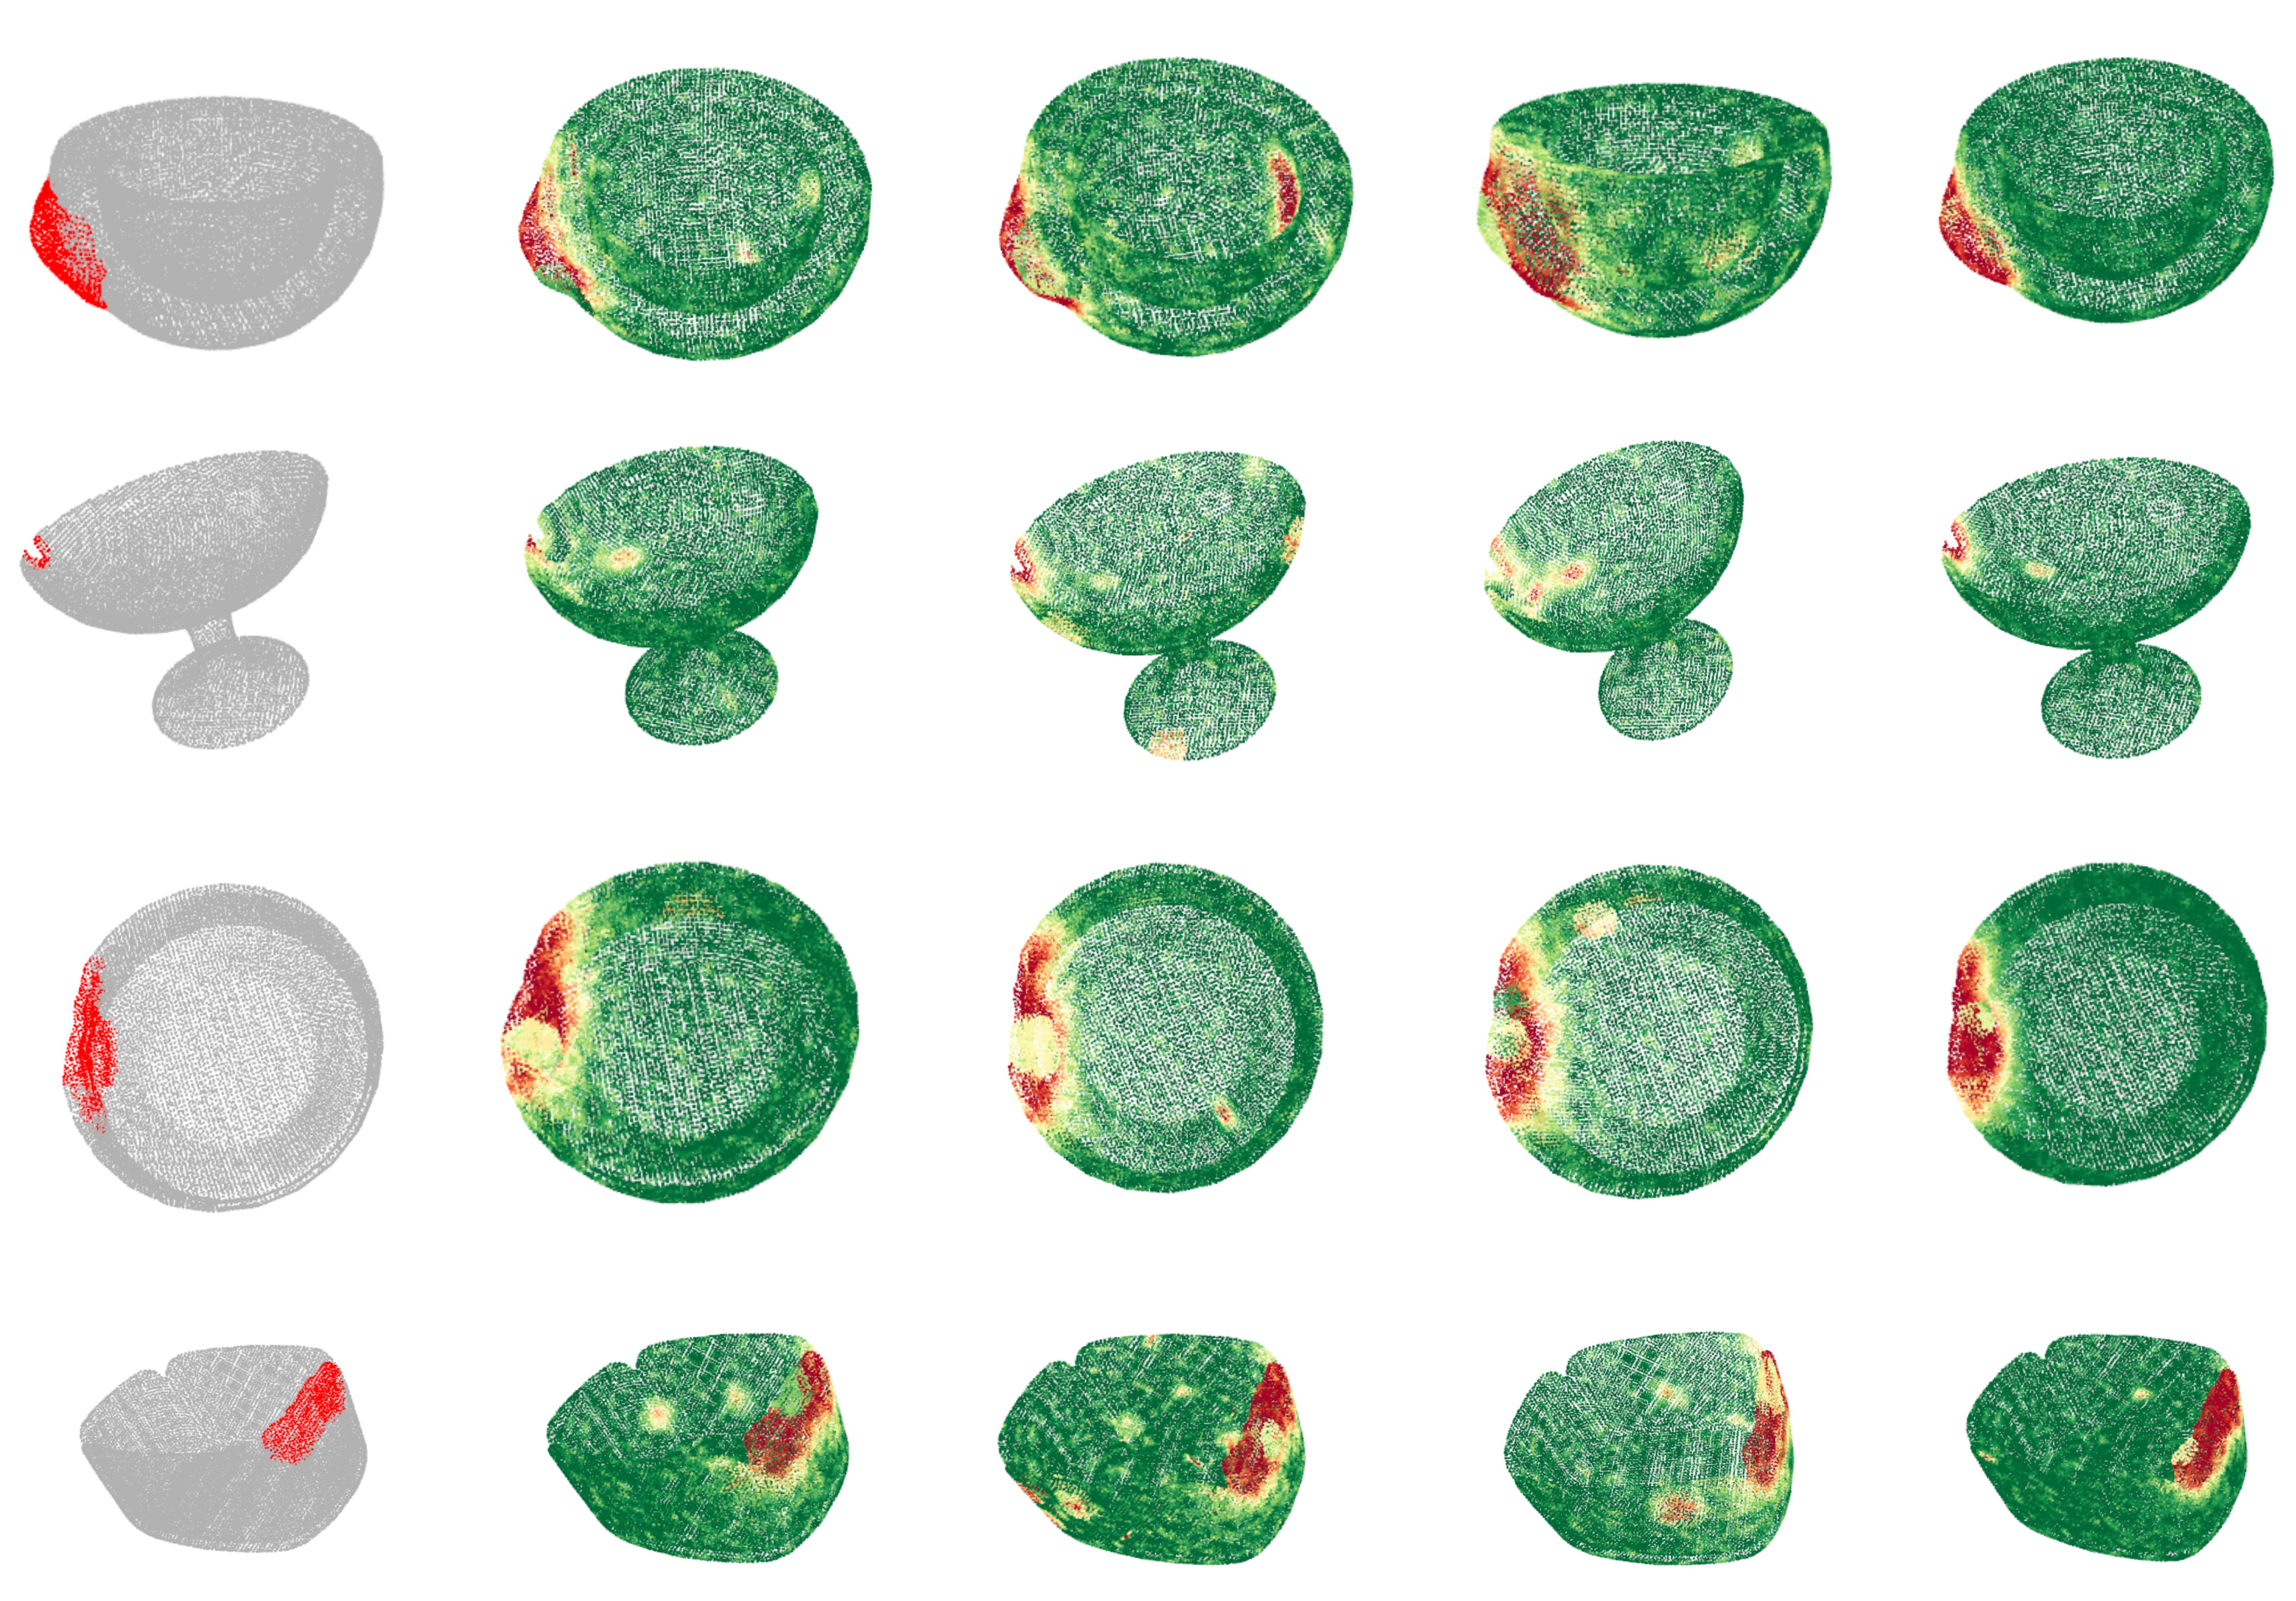
\includegraphics[width=\linewidth]{figs/shapenet}  
    Input + GT \hspace{1.2cm} 3D-ST \cite{bergmann2023anomaly} \hspace{1.3cm} Reg3D-AD \cite{liu2023real3d} \hspace{1.5cm} Group3AD   \cite{zhu2024towards} \hspace{1.7cm} Ours \hspace{0.8cm}
    \caption{Qualitative results on the newly collected Anomaly-ShapeNet \cite{li2024towards}. From left to right: input point clouds and ground truth annotations of anomalous points in red, and anomaly scores for each 3D point predicted by the proposed method.}
    \label{fig:shapenet}
\end{figure}
%-------------------------------------------------------

%-------------------------------------------------------

\begin{table}[ht]
\centering
\caption{Average Result (\%) on Anomaly-ShapeNet dataset.}
\label{tab:ShapeNet}
\begin{tabular}{l|cc|cc|c}
\hline
& \multicolumn{2}{c|}{Point Level (\%)} & \multicolumn{2}{c|}{Object Level (\%)} & Speed \\
\hline
& AUROC & AUPR & AUROC & AUPR & FPS \\ 
\hline
BTF(Raw)                            & 55.2 & 16.4  & 49.5 & 57.4  & 2.09 \\ 
BTF(FPFH)                           & 63.0 & 21.0  & 53.1 & 61.0  & 1.16 \\ 
M3DM(PointMAE)                      & 61.8 & 21.5  & 55.4 & 61.4  & 0.31 \\ 
M3DM(PointBERT)                     & 60.3 & 19.5  & 53.7 & 59.6  & 0.52 \\ 
PatchCore(FPFH)                     & 58.2 & 21.1  & 57.1 & 61.0  & 0.10 \\ 
PatchCore(FPFH+Raw)                 & 60.4 & 22.3  & 58.6 & 63.2  & 0.10 \\ 
PatchCore(PointMAE)                 & 57.9 & 19.4  & 56.4 & 59.3  & 0.12 \\ 
Reg3D-AD \cite{liu2023real3d}       & 67.0 & 20.3  & 57.4 & 70.3  & 0.10 \\ 
3D-ST \cite{bergmann2023anomaly}    & 63.6 & 22.6  & 60.7 & 60.5  & 1.52 \\
Group3AD \cite{zhu2024towards}      & 84.6 & 25.4  & 81.4 & 95.3  & 2.55 \\ 
IMRNet \cite{li2024towards}         & 65.3 & 22.8  & 66.3 & 72.7  & 5.62 \\
R3D-AD \cite{zhou2024r3d}           & 75.1 & 23.7  & 75.2 & 73.6  & 7.15 \\
Ours                                & 91.2 & 38.7  & 86.8 & 98.7  & 17.31 \\
\hline
\end{tabular}
\end{table}
%-------------------------------------------------------

Table~\ref{tab:ShapeNet} and Figure~\ref{fig:shapenet} summarize our quantitative and qualitative results on Anomaly-ShapeNet. Our method attains a point-level AUROC of 91.2\% and point-level AUPR of 38.7\%, which improves over the strongest baseline, Group3AD, by 6.6\% and 13.3\%, respectively. At the object level our AUROC is 86.8\% and AUPR is 98.7\%, exceeding Group3AD by 5.4\% and 3.4\%. These accuracy gains are achieved alongside a large runtime advantage: our default configuration runs at 17.31 FPS on the RTX-3090 workstation, which is substantially faster than the competing methods listed in Table~\ref{tab:ShapeNet}.

BTF(Raw) refers to the use of only the raw 3D coordinate features (x, y, z) within the Back-to-Front (BTF) framework \cite{horwitz2023back}. In contrast, BTF(FPFH) augments the same pipeline with Fast Point Feature Histograms (FPFH) \cite{rusu2009fast}. The entries M3DM(PointMAE) and M3DM(PointBERT) correspond to the model \cite{wang2023multimodal} configured to ignore its RGB branch and instead extract point cloud features with PointMAE \cite{pang2022masked} or PointBERT \cite{yu2022point}, respectively. For PatchCore variants, PatchCore(FPFH) replaces the usual ResNet-based feature extractor with FPFH descriptors \cite{rusu2009fast} before feeding them into the PatchCore anomaly scoring pipeline \cite{roth2022towards}. PatchCore(FPFH+Raw) further concatenates the raw spatial coordinates to each FPFH feature vector, and PatchCore(PointMAE) uses the PointMAE network \cite{pang2022masked} as the backbone feature extractor within the PatchCore framework.

The observed improvements can be traced to three design choices. First, multi-scale token fusion with the Mamba adapter aggregates complementary cues across Transformer layers so that subtle local deviations are evaluated in their broader geometric context. Defects such as bulges and concavities manifest across receptive fields and benefit from the cross-layer evidence that Mamba supplies. Second, the Geometric Semantic-Aware Sorter (GSAS) produces a geometry-preserving ordering that enables state-space fusion to propagate information along coherent surface trajectories rather than arbitrary token sequences. This geometric consistency reduces spurious contextual mixing and sharpens localization. Third, the selective anomalous feature generator provides localized, feature-space supervision that teaches the discriminator to attend to sparse, realistic deviations without corrupting global shape priors. Qualitatively, these components combine to produce compact heatmaps with low background noise for medium and large localized defects, as shown in Figure~\ref{fig:shapenet}.

Failure modes are consistent with expectations for point-based pipelines. Very thin cracks that remove only a few points remain challenging and reduce AUPR because a small number of mis-scored points strongly affects precision. High-curvature ornamental details can sometimes be mistaken for defects, which suggests that future work could incorporate curvature-aware post-processing or augment the anomalous generator with structure-preserving perturbations. Overall, the results on Anomaly-ShapeNet demonstrate that the combination of GSAS, Mamba fusion, and sparse feature-space supervision yields both state-of-the-art detection and a deployment-friendly runtime.

\subsection{Result on Real3D-AD}

%-------------------------------------------------------
\begin{figure}[!ht]
    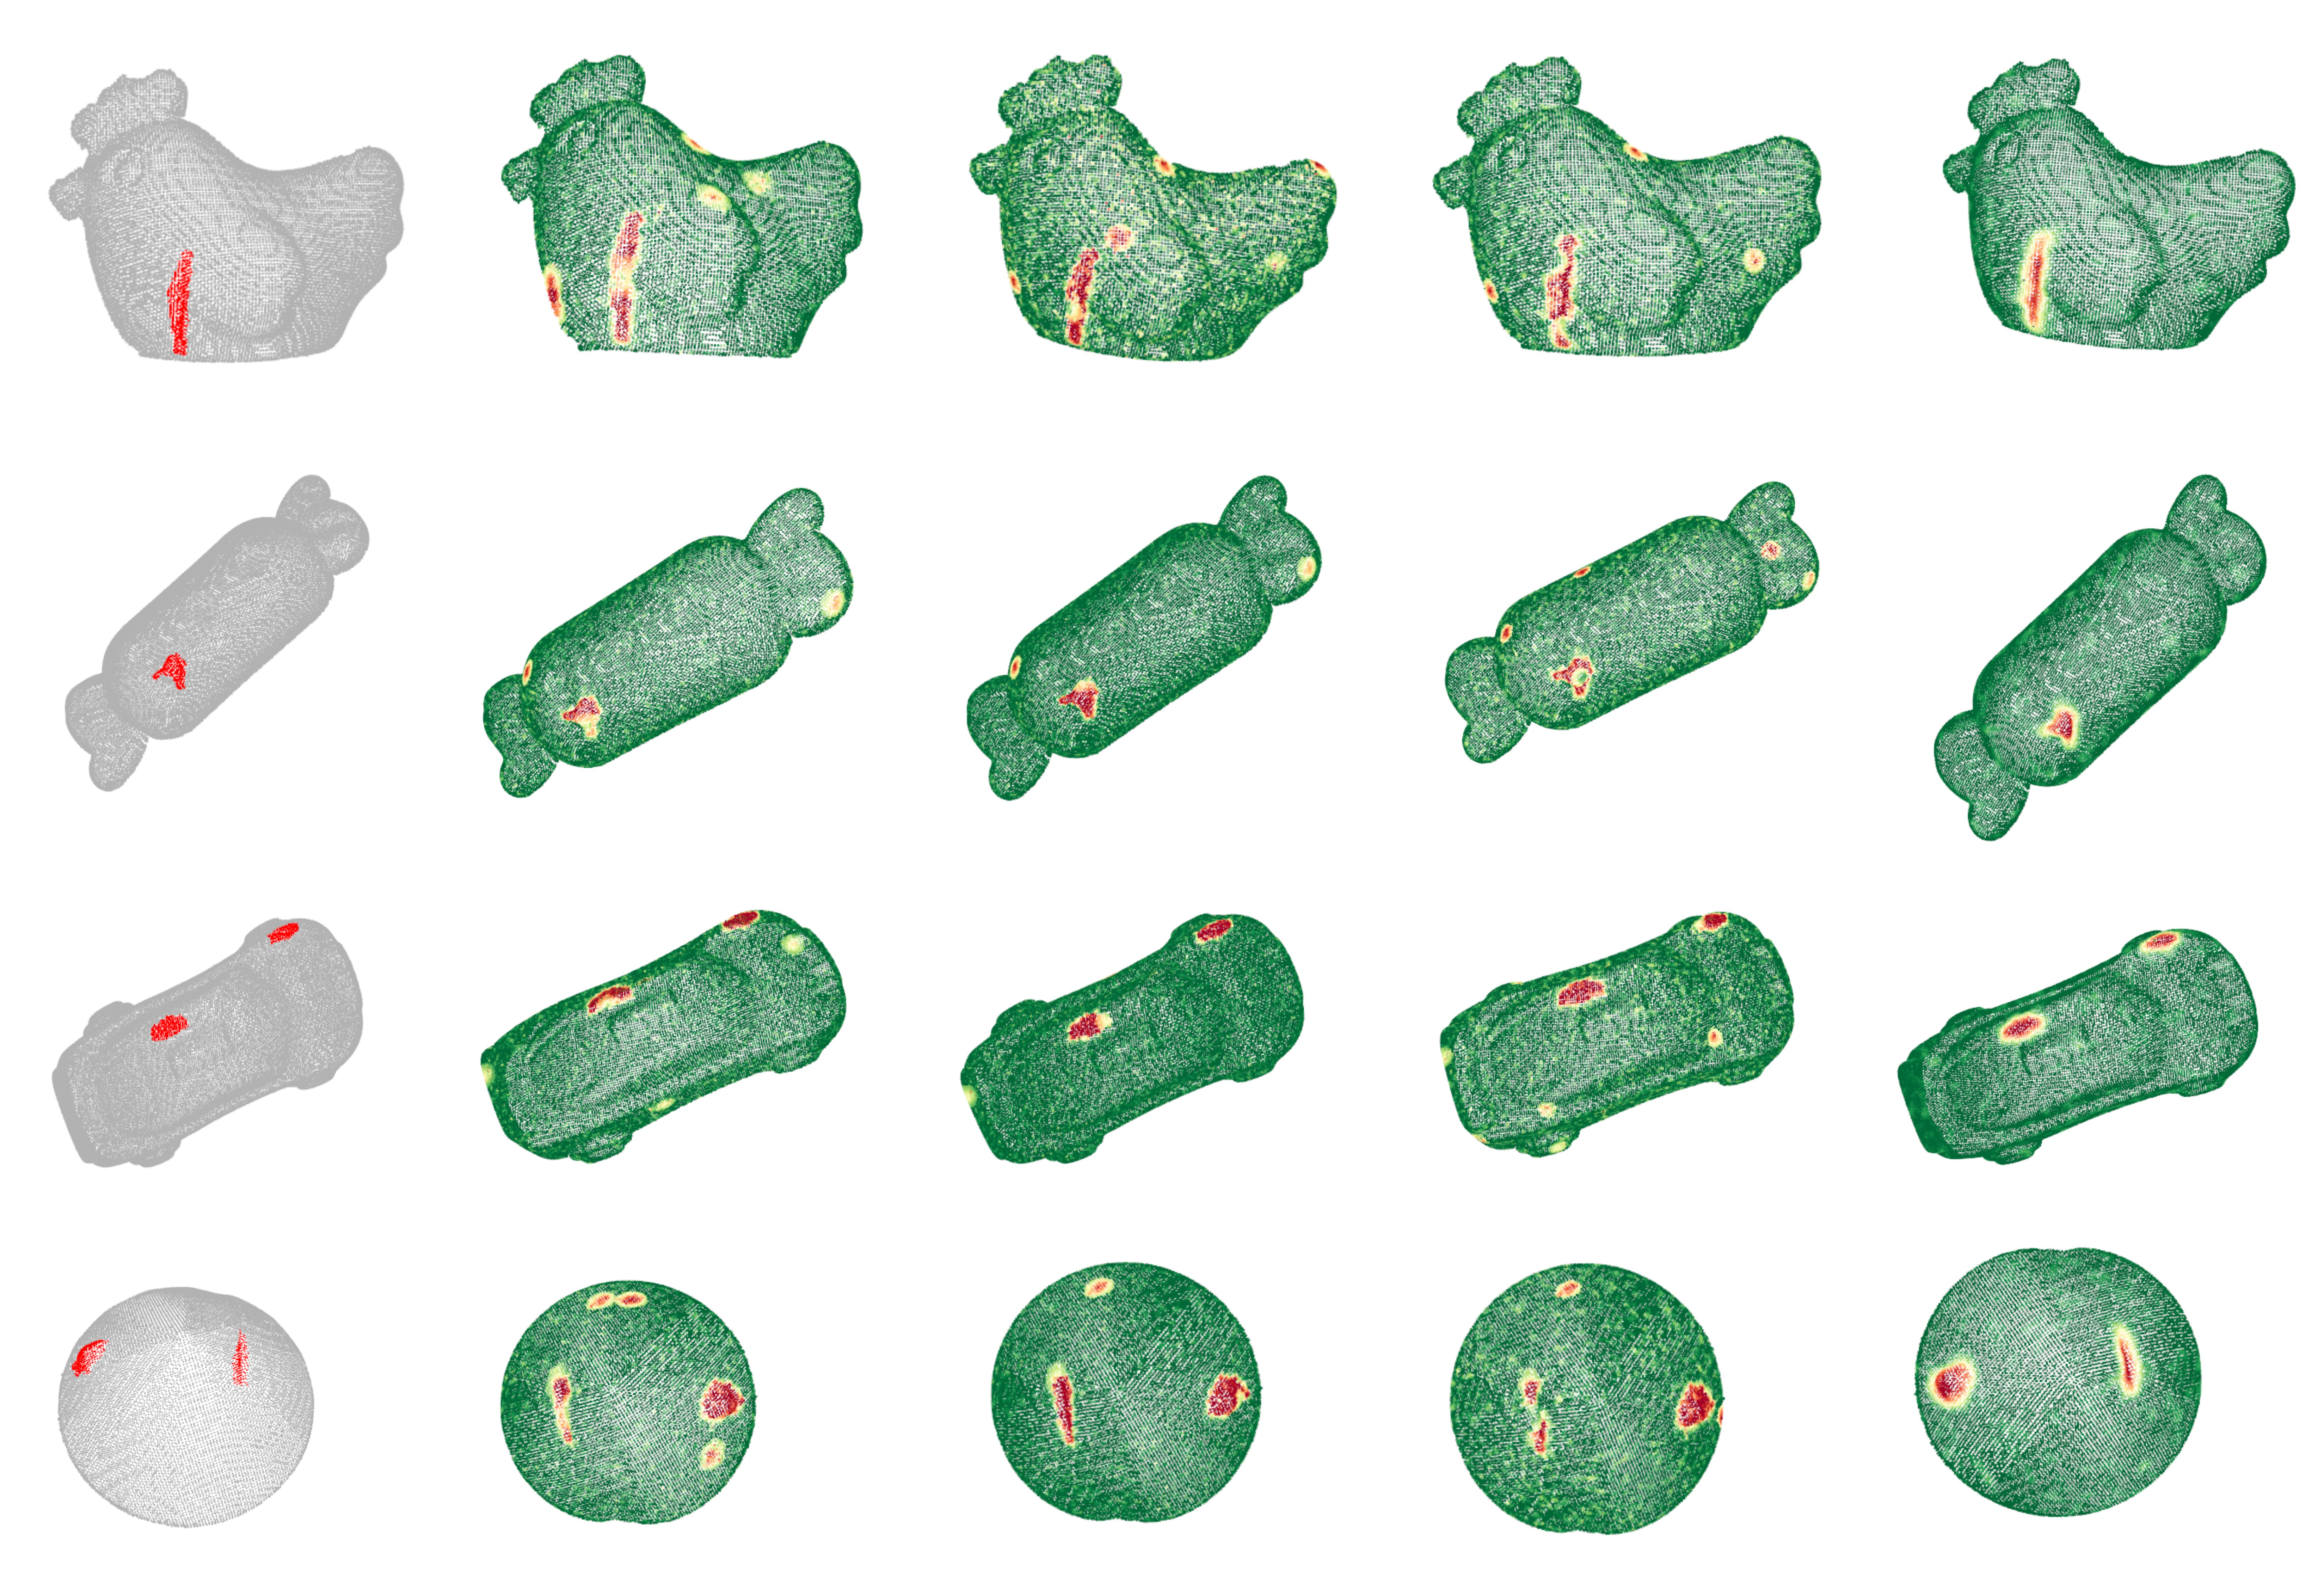
\includegraphics[width=\linewidth]{figs/real3d}
    Input + GT \hspace{1.2cm} 3D-ST \cite{bergmann2023anomaly} \hspace{1.3cm} Reg3D-AD \cite{liu2023real3d} \hspace{1.3cm} Group3AD   \cite{zhu2024towards} \hspace{1.7cm} Ours \hspace{1.5cm}
    \caption{Qualitative results on Real3D-AD dataset. From left to right: input point clouds, Ground truth annotations of anomalous points in red, and anomaly scores for each 3D point predicted by the proposed method.}
    \label{fig:real3d}
\end{figure}
%-------------------------------------------------------

%-------------------------------------------------------

\begin{table}[ht]
\centering
\caption{Average Results (\%) on Real3D-AD dataset.}
\label{tab:Real3D}
\begin{tabular}{l|cc|cc|c}
\hline
& \multicolumn{2}{c|}{Point Level (\%)} & \multicolumn{2}{c|}{Object Level (\%)} & Speed \\
\hline
& AUROC & AUPR & AUROC & AUPR & FPS \\ 
\hline
BTF(Raw)                            & 57.3 & 2.4 & 60.5 & 61.3  & 2.05 \\
BTF(FPFH)                           & 73.2 & 6.6 & 63.7 & 61.6  & 1.01 \\
M3DM(PointMAE)                      & 63.9 & 4.9 & 55.4 & 57.5  & 0.31 \\
M3DM(PointBERT)                     & 63.9 & 5.4 & 54.0 & 58.3  & 0.52 \\
PatchCore(FPFH)                     & 57.9 & 7.3 & 59.6 & 59.3  & 0.10 \\
PatchCore(FPFH+Raw)                 & 68.2 & 12.5 & 68.4 & 66.9  & 0.10 \\
PatchCore(PointMAE)                 & 64.5 & 6.0 & 59.6 & 63.6  & 0.12 \\
Reg3D-AD \cite{liu2023real3d}       & 70.7 & 11.1 & 70.7 & 72.6  & 0.10 \\
3D-ST \cite{bergmann2023anomaly}    & 70.7 & 11.1 & 64.8 & 72.6  & 1.52 \\
Group3AD   \cite{zhu2024towards}    & 73.8 & 13.9 & 75.3 & 74.3  & 2.55 \\
IMRNet   \cite{li2024towards}       & 72.8 & 16.8 & 72.8 & 62.8  & 5.62 \\
R3D-AD   \cite{zhou2024r3d}         & 59.4 & 4.3 & 73.6 & 63.5  & 7.15 \\
Ours                                & 76.6 & 19.7 & 78.4 & 77.7 & 17.31 \\
\hline
\end{tabular}
\end{table}

%-------------------------------------------------------

Table~\ref{tab:Real3D} and Figure~\ref{fig:real3d} report performance on Real3D-AD, where scans are high density and defects arise under realistic sensor conditions. We compare with the same set of state-of-the-art methods used for Anomaly-ShapeNet. Our method achieves a point-level AUROC of 76.6\% and point-level AUPR of 19.7\%, improving over Group3AD by 2.8\% and 5.8\%, respectively. At the object level we obtain an AUROC of 78.4\% and an AUPR of 77.7\%, improving over Group3AD by 3.1\% and 3.4\%. As on the synthetic benchmark, our approach maintains a large throughput advantage with 17.31 FPS, which supports practical deployment in industrial inspection pipelines. Real3D-AD differs from synthetic benchmarks in three ways that highlight the strengths of our design. First, defects in real scans are often subtle and must be discriminated from sensor noise and varying point density. Mamba fusion aggregates multi-layer signals so that local irregularities are evaluated with respect to global part geometry, which reduces false positives caused by sensor artifacts. Second, GSAS ensures that the fusion operates on a surface-aware ordering, which is important in dense, complex scans to prevent unrelated surface regions from contaminating contextual cues. Third, the selective anomalous feature generator produces spatially sparse supervisory signals that encourage sensitivity to small but consistent deviations, which is useful when prototype sets are limited and supervised defect examples are scarce.

Qualitatively, our method reliably highlights dents, missing material, and other geometric defects with high contrast while keeping false detections low in benign regions. Limitations include reduced sensitivity to appearance-only anomalies that do not affect geometry and occasional loss of localization precision in heavily occluded or extremely unevenly sampled areas. Practical mitigations include fusing appearance or reflectance channels when available and applying local density normalization during preprocessing. Results on Real3D-AD corroborate the conclusions from the synthetic benchmark. The combination of geometry-preserving ordering, linear-time cross-layer fusion, and sparse feature-space supervision improves both detection and localization robustness while offering a favorable runtime and memory profile for industrial applications.

\subsection{Ablation Study}


\section{Conclusion}

